\documentclass[11pt,a4paper]{article}
\usepackage[utf8]{inputenc}
\usepackage[T1]{fontenc}
\usepackage{lmodern}
\usepackage[margin=2.5cm]{geometry}
\usepackage{booktabs}
\usepackage{graphicx}
\usepackage{caption}
\usepackage{float}
\usepackage{amsmath}
\usepackage{breqn}
\usepackage[hidelinks]{hyperref}

\title{An automatic report for the dataset: 05-temperature}
\author{\texttt{autostat} (automatic-statistician-revisited)}
\date{08 November 2026}

\begin{document}
\maketitle

\noindent\emph{Produced by \texttt{autostat}, a Python 3 port of the Automatic Bayesian Covariance Discovery system of Lloyd et al. (AAAI 2014).}


\begin{figure}[H]
\centering
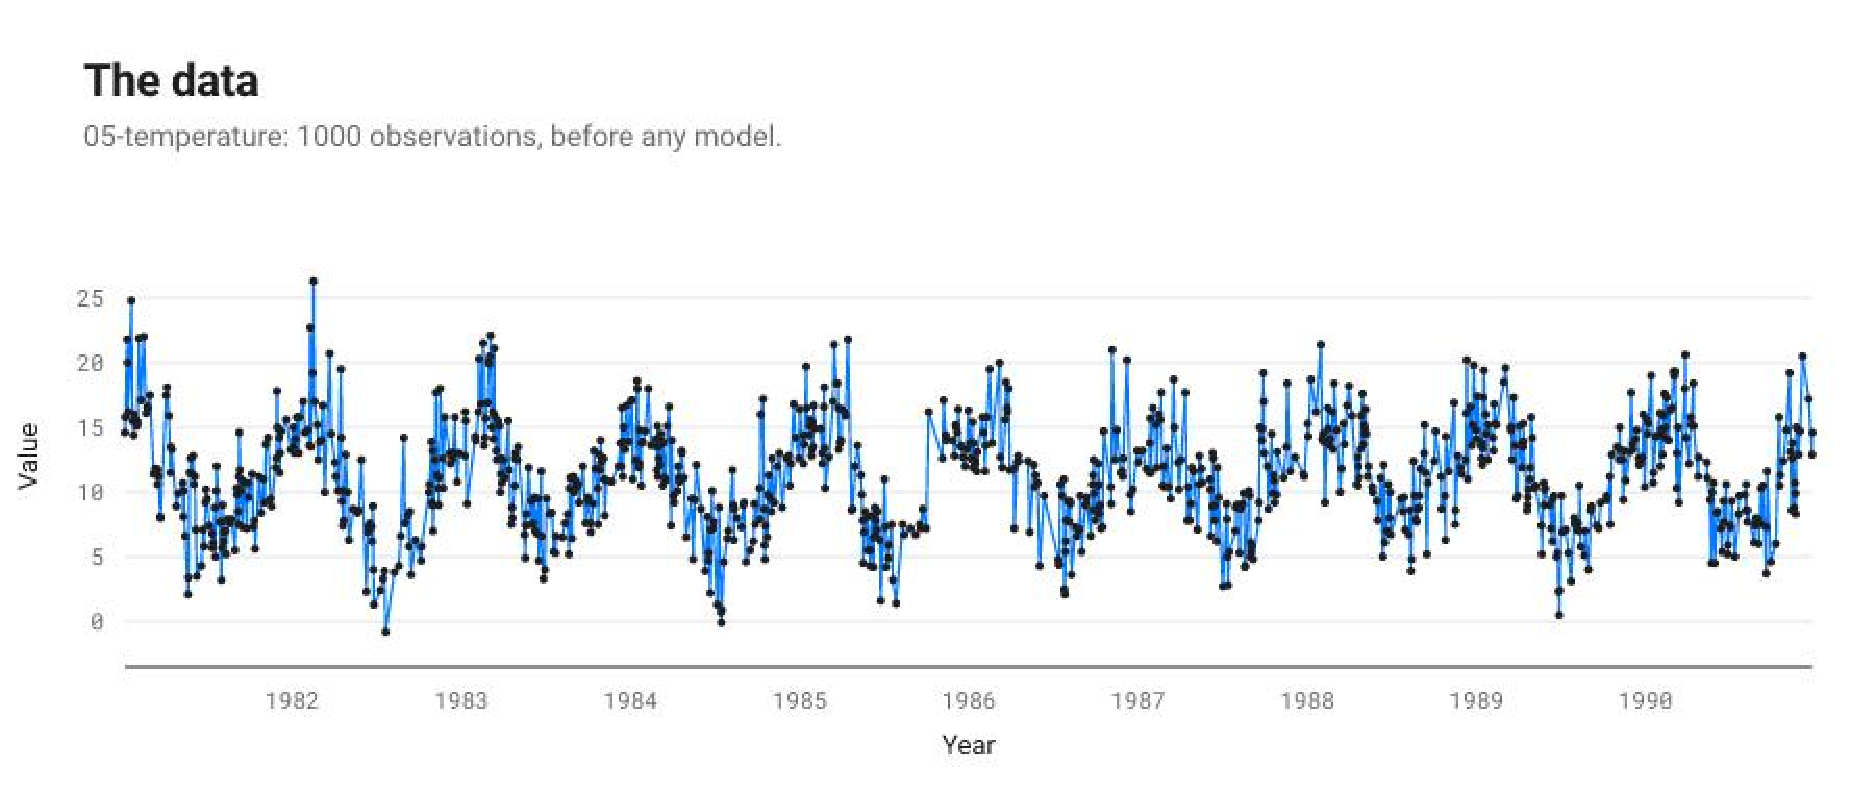
\includegraphics[width=\linewidth]{data.pdf}
\caption*{The data}
\end{figure}

\section*{Executive summary}

The structure search selected \texttt{C + WN + Per + SE} (Bayesian information criterion 4828.7; negative log likelihood 2390.2 on 1000 points). It decomposes into 4 additive components, listed by how much each reduces extrapolation error:
\begin{enumerate}
  \item A constant.
  \item A periodic function with a period of 1.0 years.
  \item A rapidly varying smooth function.
  \item Uncorrelated noise.
\end{enumerate}

\begin{center}
\begin{tabular}{lrrrr}
\toprule
\# & $R^2$ cumulative (\%) & Residual variance explained (\%) & CV MAE & MAE reduction (\%) \\
\midrule
data & & & 11.2 & \\
1 & 0.0 & 0.0 & 3.34 & 70.2 \\
2 & 54.6 & 54.6 & 2.23 & 33.4 \\
3 & 97.8 & 95.1 & 2.22 & 0.1 \\
4 & 100.0 & 100.0 & 2.22 & 0.0 \\
\bottomrule
\end{tabular}
\end{center}

MAE: mean absolute error over ten contiguous held-out blocks; CV: cross-validated.

\section*{The formula found}

The structure search is a symbolic regression: it searches a grammar of expressions over kernels and keeps the one with the lowest Bayesian information criterion. This is the expression it kept, with every fitted parameter in place; $t$ is in years.
\begin{dmath*}
y(t) = f_{1}(t) + f_{2}(t) + f_{3}(t) + f_{4}(t)
\end{dmath*}

Each component is a Gaussian process with its own covariance:
\begin{dmath*}
f_{1}(t) \sim \mathrm{GP}\!\left(0,\ 147.7\right)
\end{dmath*}
\begin{dmath*}
f_{2}(t) \sim \mathrm{GP}\!\left(0,\ 7.967\,\frac{\exp\!\left(0.1033\cos\frac{2\pi (t - t')}{1.001}\right) - I_0(0.1033)}{e^{0.1033} - I_0(0.1033)}\right)
\end{dmath*}
\begin{dmath*}
f_{3}(t) \sim \mathrm{GP}\!\left(0,\ 6.432\,\exp\!\left(-\frac{(t - t')^2}{2 \cdot 0.003448^2}\right)\right)
\end{dmath*}
\begin{dmath*}
f_{4}(t) \sim \mathrm{GP}\!\left(0,\ 1.459\,\delta_{t t'}\right)
\end{dmath*}

These components have a closed form, read from their posterior mean:
\begin{dmath*}
f_{1}(t) = 11.15
\end{dmath*}
\begin{dmath*}
f_{2}(t) \approx 4.293\cos\!\left(\frac{2\pi \cdot (t - 1981)}{1.001} - 0.3861\right) + 0.5723\cos\!\left(\frac{2\pi \cdot 2 \cdot (t - 1981)}{1.001} - 2.754\right) + 0.009047\cos\!\left(\frac{2\pi \cdot 3 \cdot (t - 1981)}{1.001} + 1.623\right)
\end{dmath*}

A periodic kernel is exactly a sum of cosines, so a periodic component is a Fourier series in its period; it is written up to the harmonic after which the rest weighs less than 0.1 % of the component, hence the approximate sign.

The other components are smooth, quasi-periodic or noise without a short formula: a draw from such a process has no finite closed form; its covariance above is the formula.

Closed form of each component:

\begin{center}\footnotesize
\begin{tabular}{lp{0.36\linewidth}l}
\toprule
\# & component & closed form \\
\midrule
1 & A constant & exact polynomial of degree 0 \\
2 & A periodic function with a period of 1.0 years & Fourier series, 3 harmonics, largest gap 0.011 \% of the component \\
3 & A rapidly varying smooth function & none: the covariance is the formula \\
4 & Uncorrelated noise & none: the covariance is the formula \\
\bottomrule
\end{tabular}
\end{center}

\section*{Search path and stopping criterion}

The 2014 configuration searches a fixed number of levels and keeps the lowest BIC; it has no stopping rule. The table follows the winner of each level. A change of structure adds or removes terms; a level that keeps the structure only refits its parameters. BIC differences read on the scale of Kass and Raftery (1995): under 2 barely worth mentioning, 2 to 6 positive, 6 to 10 strong, over 10 very strong.

\begin{center}\footnotesize
\begin{tabular}{lllp{0.36\linewidth}lll}
\toprule
level & BIC & change & structure & components & closed & params \\
\midrule
1 & 5038.5 &  & WN + SE & 2 & 0 & 3 \\
2 & 4985.2 & -53.3 & WN + Per + SE & 3 & 1 & 6 \\
3 & 4955.6 & -29.6 & WN + Per + Per x SE + SE + SE & 5 & 1 & 12 \\
4 & 4845.2 & -110.4 & WN + Per + SE + SE & 4 & 1 & 8 \\
5 & 4833.9 & -11.3 & C + Per + SE & 3 & 2 & 6 \\
6 & 4829.5 & -4.4 & C + WN + Per + SE & 4 & 2 & 7 \\
7 & 4828.8 & -0.7 & C + WN + Per + SE & 4 & 2 & 7 \\
8 & 4828.8 & +0.0 & C + WN + Per + SE & 4 & 2 & 7 \\
9 (kept) & 4828.7 & -0.1 & C + WN + Per + SE & 4 & 2 & 7 \\
10 & 4828.7 & +0.0 & C + WN + Per + SE & 4 & 2 & 7 \\
\bottomrule
\end{tabular}
\end{center}

\begin{figure}[H]
\centering
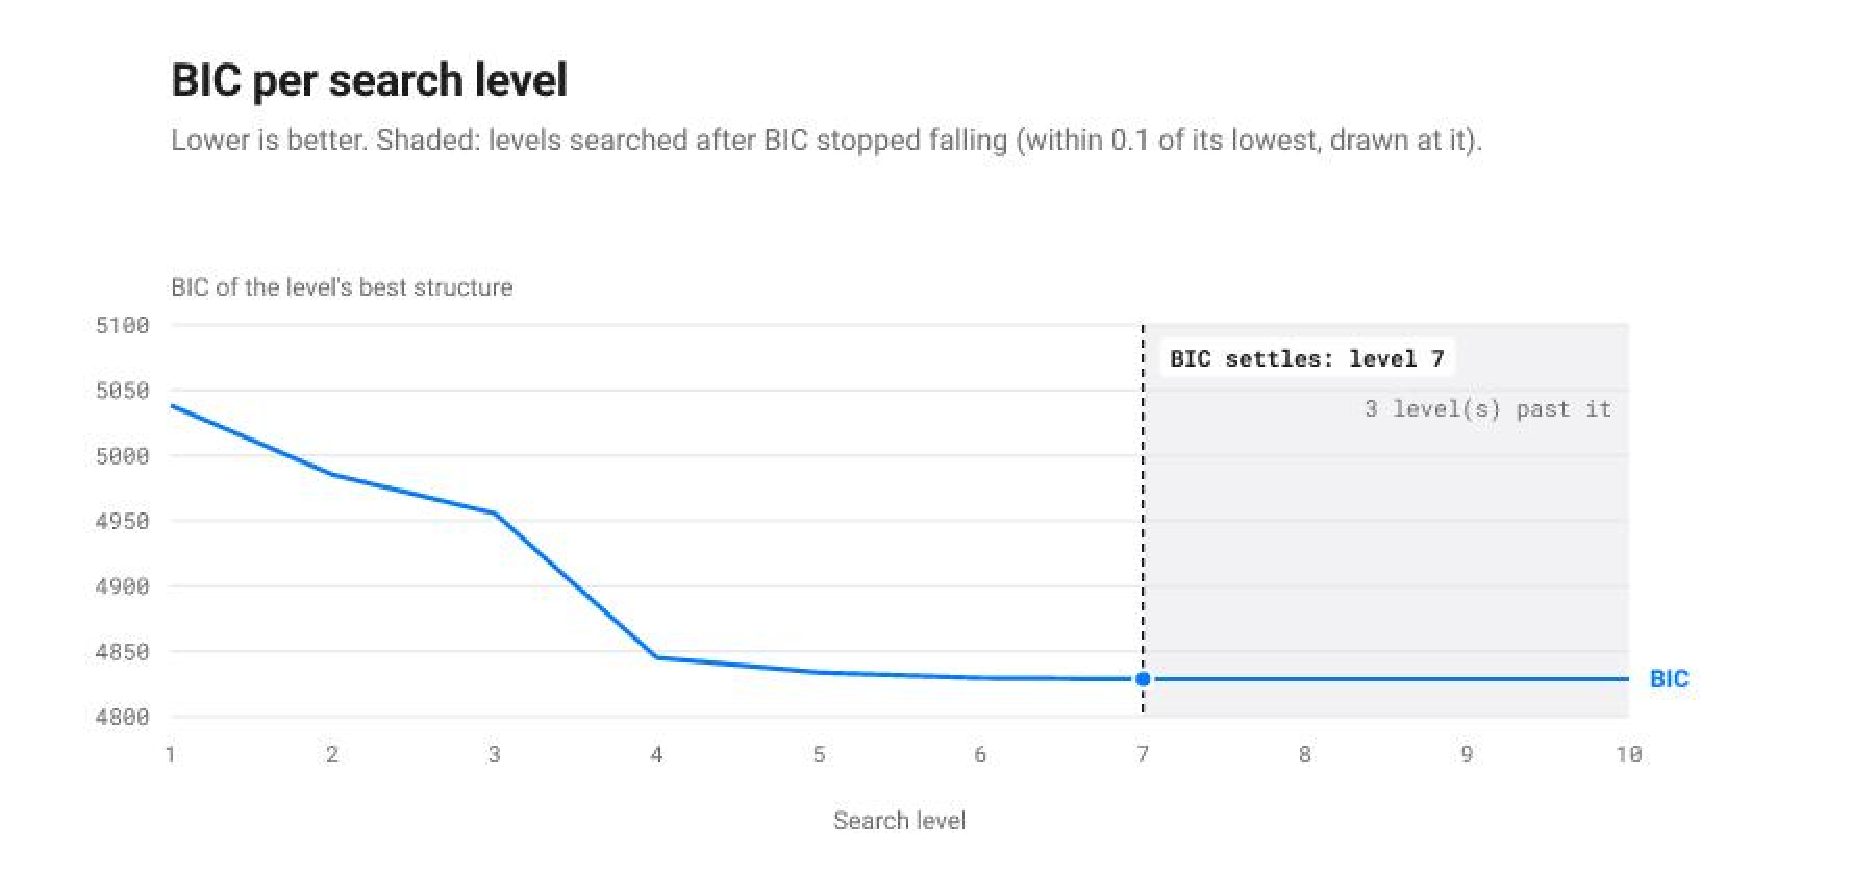
\includegraphics[width=\linewidth]{bic.pdf}
\caption*{BIC per search level}
\end{figure}

\begin{itemize}
\item The search ran 10 levels (the published 2014 search: ten levels, no stopping rule) and keeps the model of level 9, C + WN + Per + SE, BIC 4828.7.
\item That structure was first reached at level 6; the levels after it only refitted its parameters, lowering BIC by 0.8 in all.
\item The best different structure, C + Per + SE (level 5), is 5.2 above it: positive evidence for the kept one on the Kass and Raftery scale.
\item BIC stopped falling at level 7. The 3 level(s) searched past it kept its structure and lowered BIC by 0.09 in all, less than the tolerance of 0.1: going on buys nothing the data pay for.
\item A rule stopping after 1 level(s) without a fall above 0.1 would have ended the search at level 8 and kept the same structure, less refitted.
\item A rule stopping after 2 level(s) without a fall above 0.1 would have ended the search at level 9 and kept the same model.
\item The kept expression has 7 parameters for 1000 points: its BIC is a fit term 2 NLL = 4780.3 plus a complexity term p ln n = 48.4, each extra parameter costing 6.91; it splits into 4 components, 2 of them with a closed form.
\end{itemize}

\begin{figure}[H]
\centering
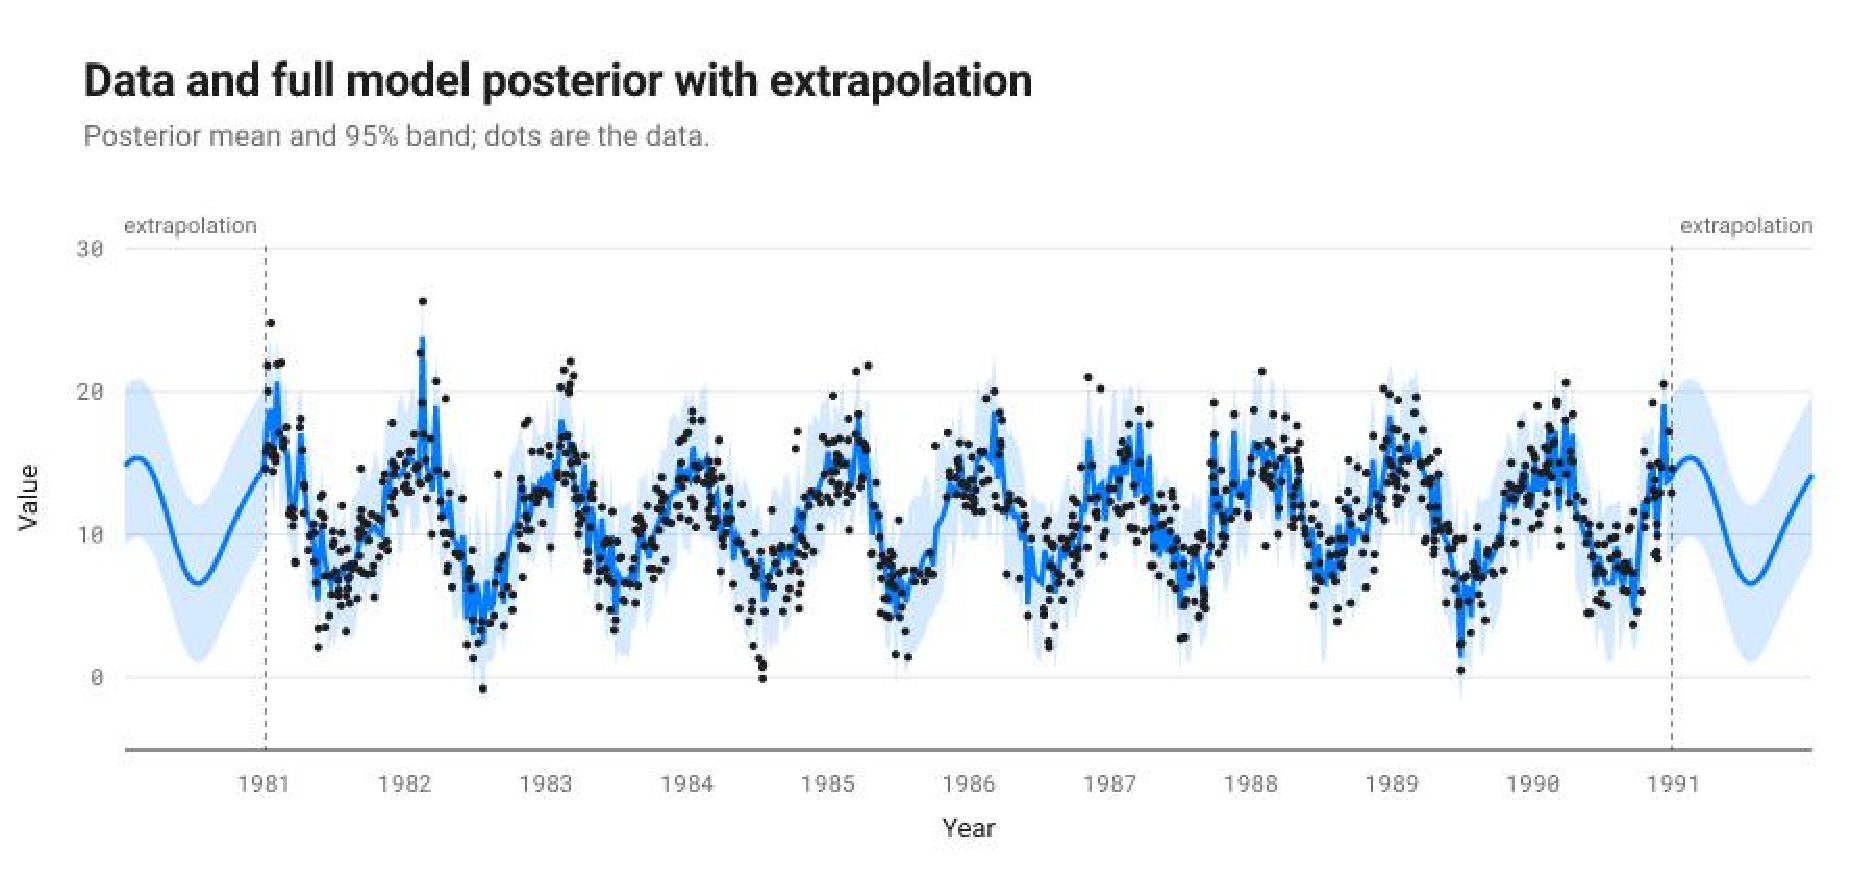
\includegraphics[width=\linewidth]{fit.pdf}
\caption*{Data and full posterior}
\end{figure}

\section*{Detailed discussion of the components}

\subsection*{Component 1: A constant}

This component is constant.

This component explains 0.0\% of the data's variance on its own; with the components above it, 0.0\%. Adding it changes the cross-validated MAE by -70.2\%.

\emph{Extrapolation.} This component is assumed to stay constant.

\begin{figure}[H]
\centering
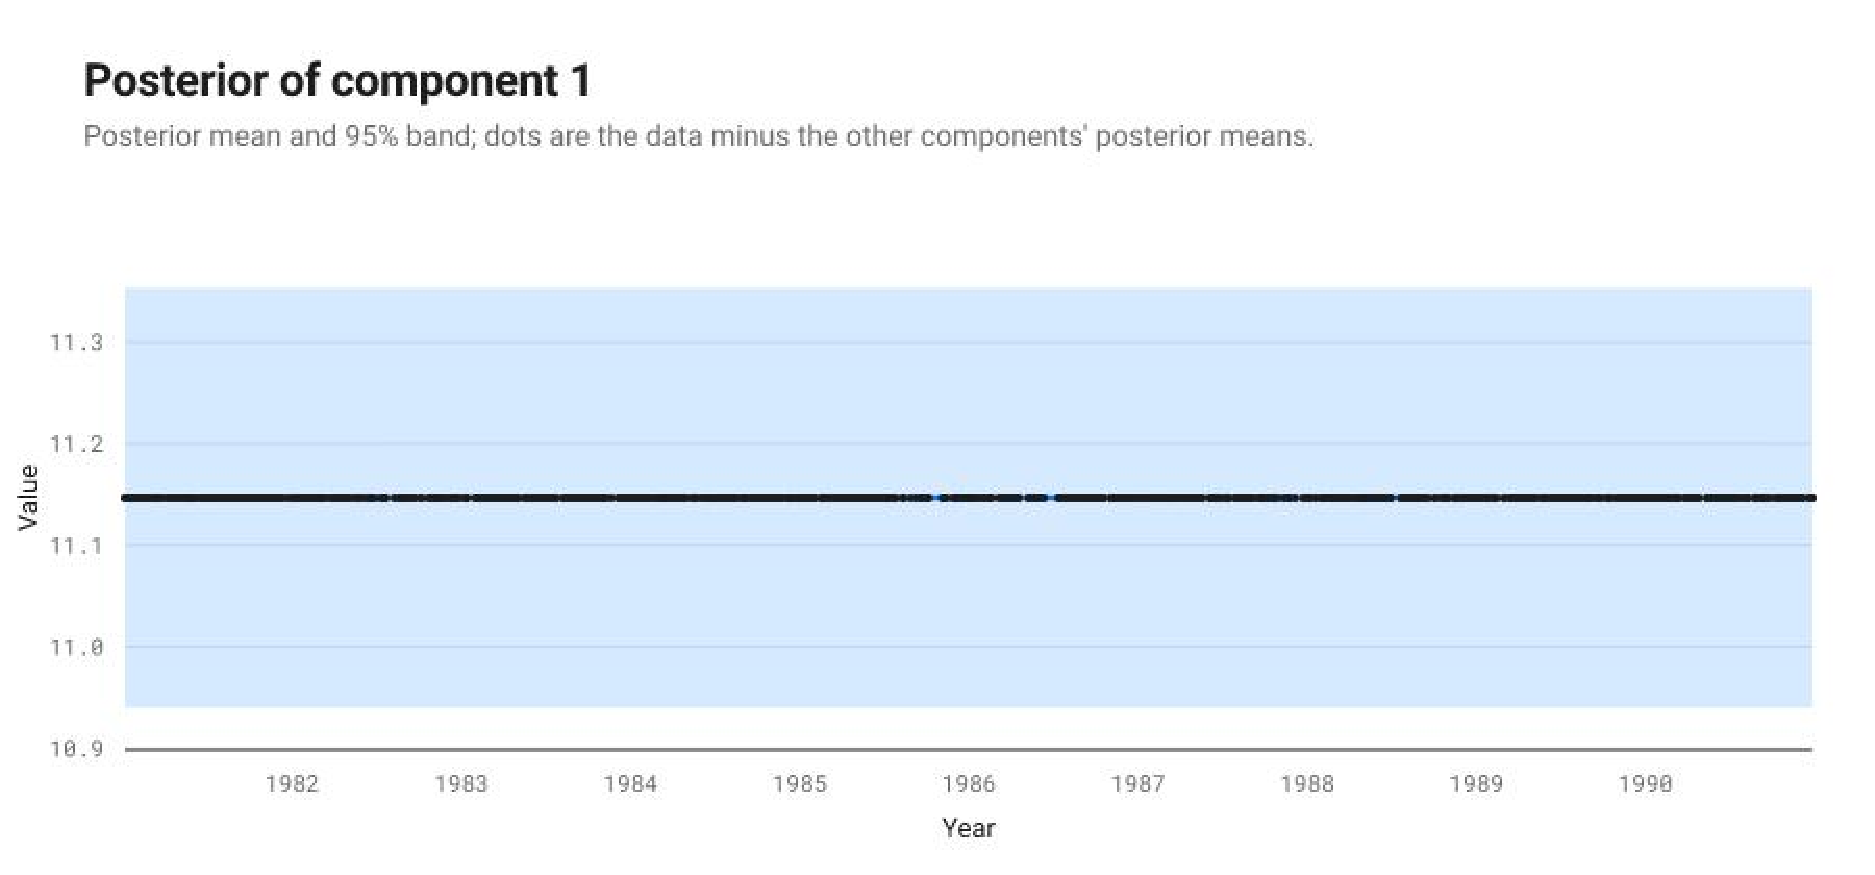
\includegraphics[width=\linewidth]{component_1.pdf}
\caption*{Component 1}
\end{figure}
\subsection*{Component 2: A periodic function with a period of 1.0 years}

This component is periodic with a period of 1.0 years. The shape of this function within each period has a typical lengthscale of 5.9 months.

This component explains 54.6\% of the data's variance on its own; with the components above it, 54.6\%. Adding it changes the cross-validated MAE by -33.4\%.

\emph{Extrapolation.} This component is assumed to continue periodically with a period of 1.0 years.

\begin{figure}[H]
\centering
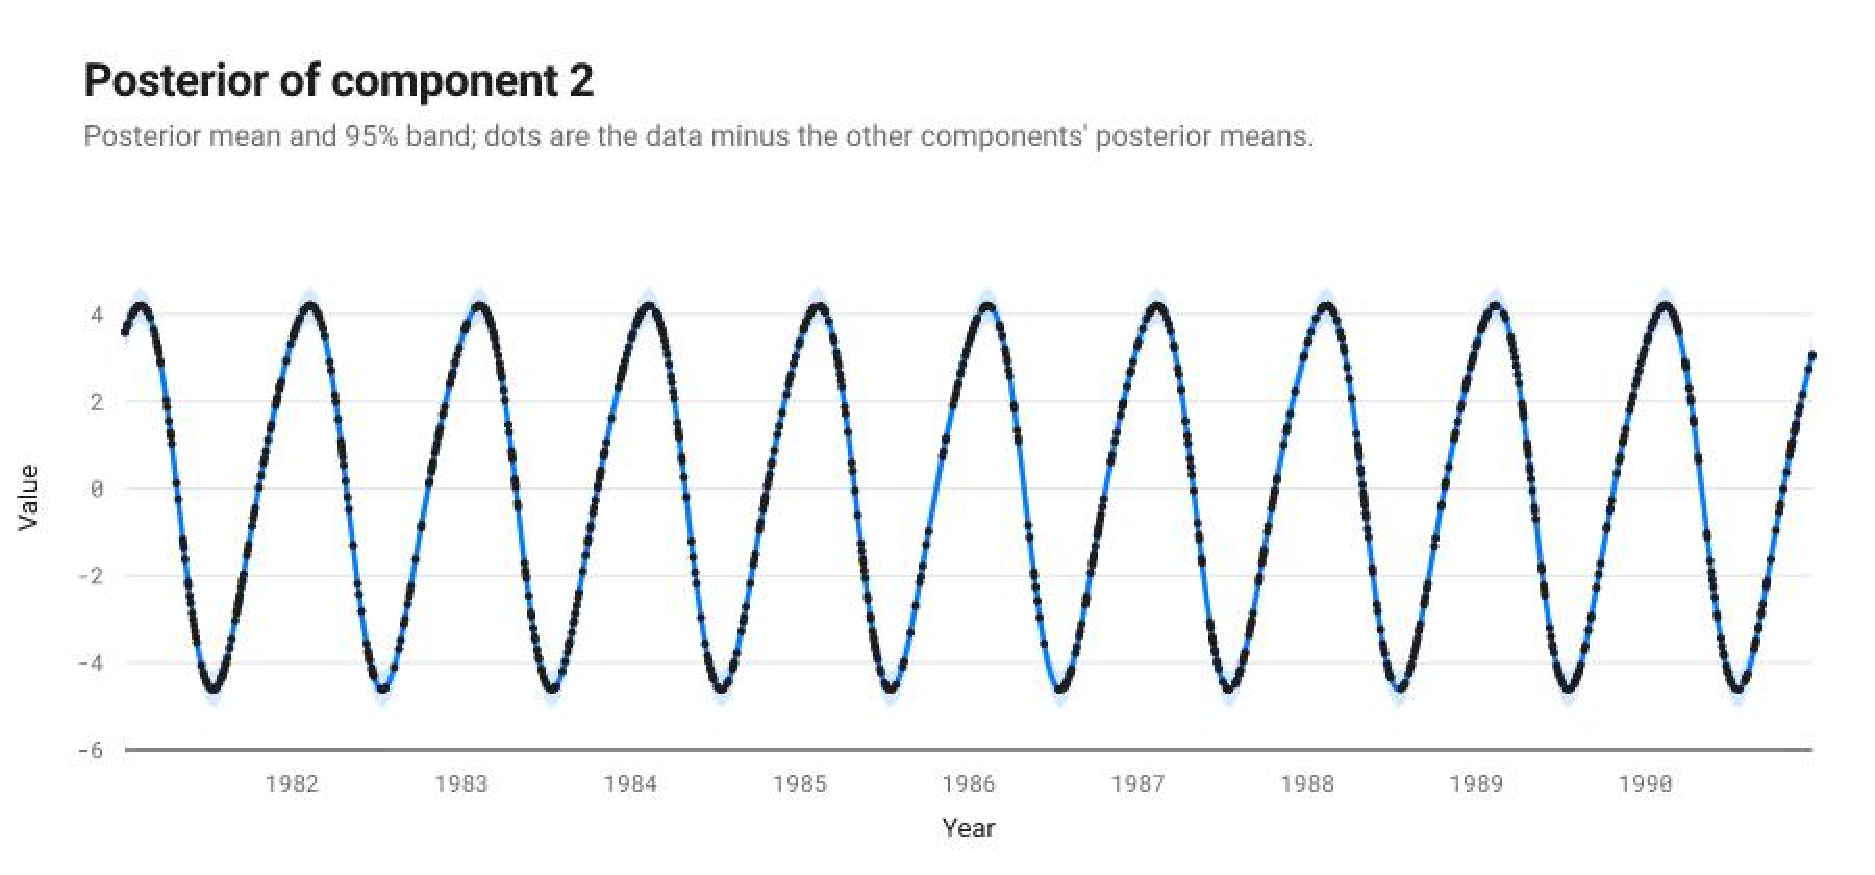
\includegraphics[width=\linewidth]{component_2.pdf}
\caption*{Component 2}
\end{figure}
\subsection*{Component 3: A rapidly varying smooth function}

This component is a rapidly varying but smooth function with a typical lengthscale of 30.2 hours.

This component explains 41.8\% of the data's variance on its own; with the components above it, 97.8\%. Adding it changes the cross-validated MAE by -0.1\%.

\emph{Extrapolation.} This component is assumed to continue smoothly but its distribution is assumed to quickly return to the prior. The prior distribution places mass on smooth functions with a marginal mean of zero and a typical lengthscale of 30.2 hours.

\begin{figure}[H]
\centering
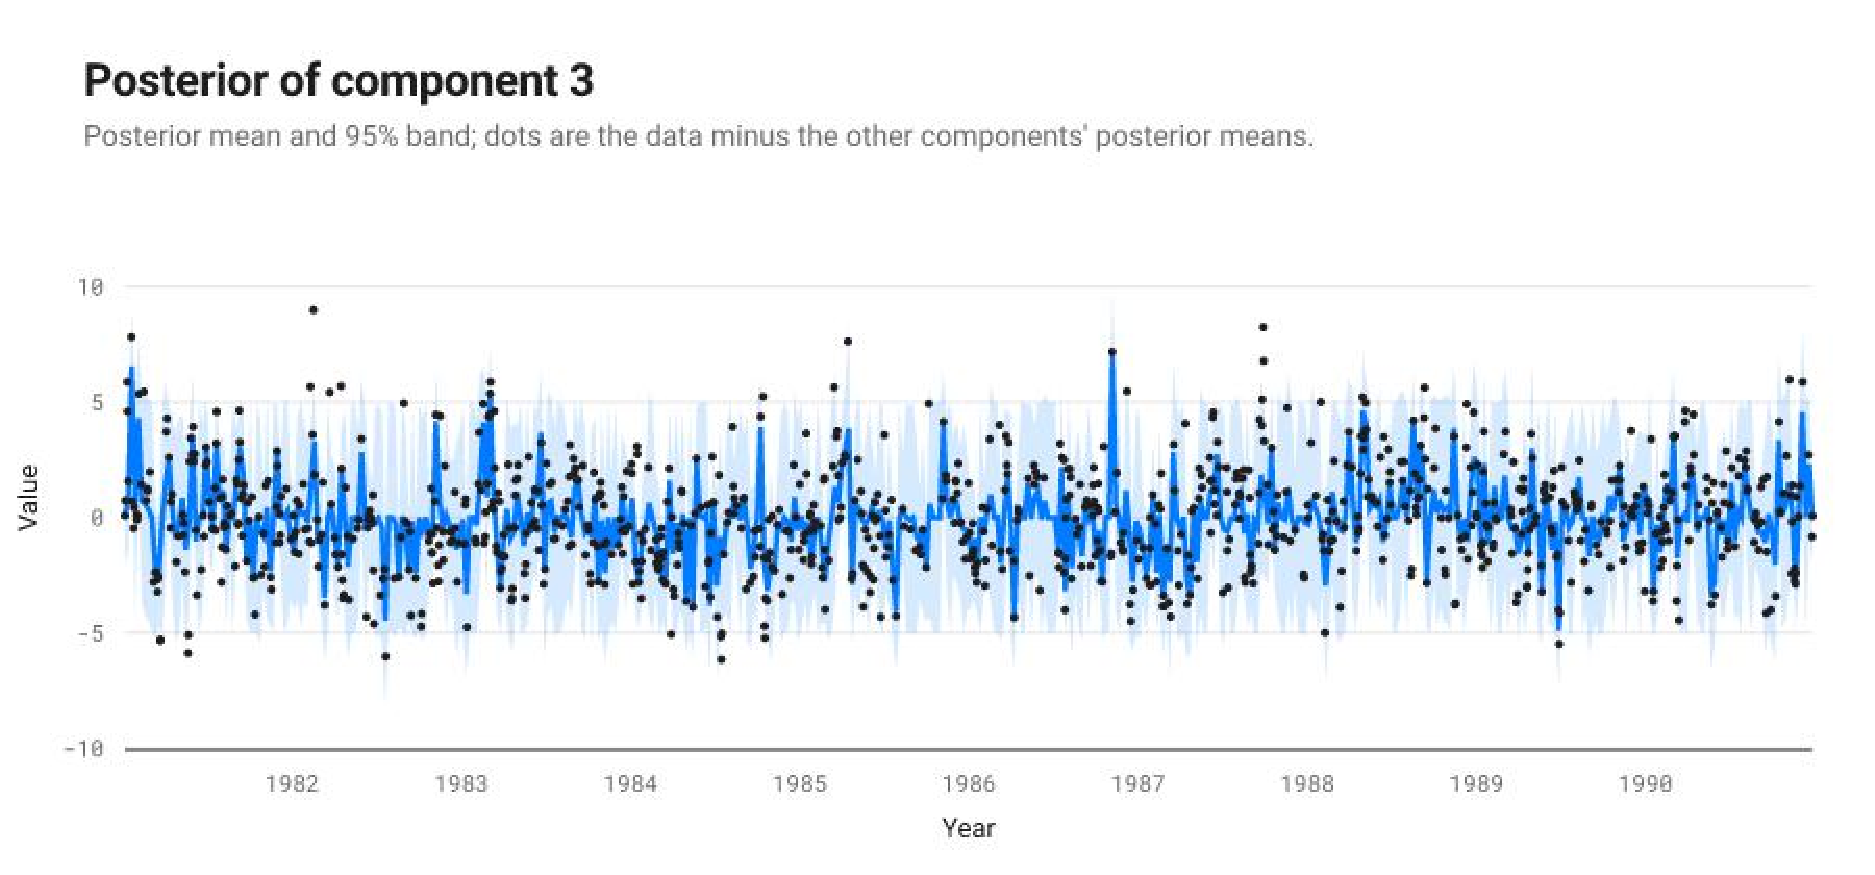
\includegraphics[width=\linewidth]{component_3.pdf}
\caption*{Component 3}
\end{figure}
\subsection*{Component 4: Uncorrelated noise}

This component models uncorrelated noise.

This component explains 14.8\% of the data's variance on its own; with the components above it, 100.0\%. Adding it changes the cross-validated MAE by -0.0\%.

\emph{Extrapolation.} This component assumes the uncorrelated noise will continue indefinitely.

\begin{figure}[H]
\centering
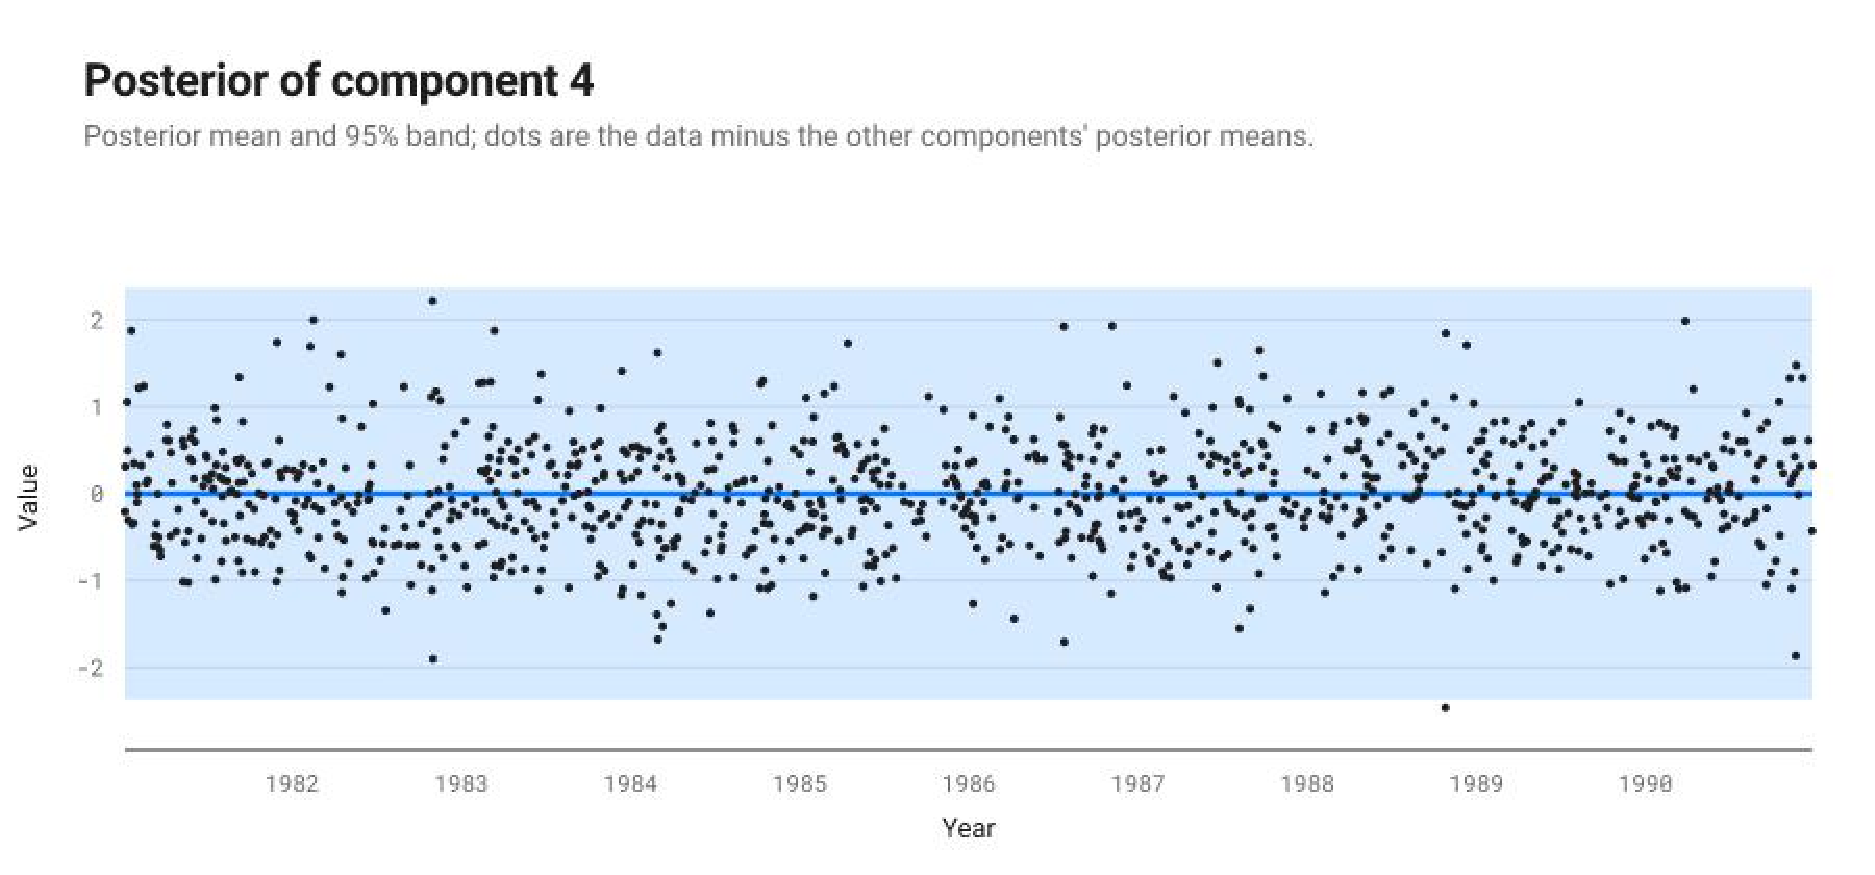
\includegraphics[width=\linewidth]{component_4.pdf}
\caption*{Component 4}
\end{figure}

\section*{Model checking}

Each statistic compares draws of a component's posterior with draws of its prior. A small p-value (bold below 0.05) points at a property of the data that the component's prior does not reproduce.

\begin{center}
\begin{tabular}{lrrrrrrr}
\toprule
\# & QQ max & QQ min & ACF min & ACF min lag & Pgram max & Pgram peak & MMD \\
\midrule
1 & 0.330 & 0.330 & 0.986 & 0.952 & 0.728 & 0.966 & \textbf{0.000} \\
2 & 0.508 & 0.680 & 0.876 & 0.460 & 0.646 & 0.990 & \textbf{0.000} \\
3 & 0.214 & 0.280 & 0.906 & 0.772 & 0.894 & 0.734 & \textbf{0.000} \\
4 & 0.834 & 0.896 & 0.992 & 0.990 & 0.954 & 0.998 & \textbf{0.000} \\
\bottomrule
\end{tabular}
\end{center}

QQ: quantile-quantile gaps. ACF: autocorrelation function. Pgram: periodogram. MMD: maximum mean discrepancy two-sample test.

\end{document}
